\documentclass{polyu-comp}
\usepackage[T1]{fontenc}
\usepackage{tabularx} % For tables with adjustable columns
\usepackage{url}
\usepackage{booktabs}
\usepackage{graphicx}
\usepackage{algorithm}
\usepackage{algorithmic}
\usepackage{tikz}
\usetikzlibrary{shapes.geometric, arrows.meta, positioning, fit, calc}
\usepackage[absolute]{textpos}
\usepackage{listings}
\usepackage{amssymb}
\usepackage{amsmath}
\usepackage{titlesec}
\usepackage[table]{xcolor} % 用于表格行背景色
\newcolumntype{Y}{>{\centering\arraybackslash}X}
\newcommand{\sectionbreak}{\clearpage}

\lstset{
    basicstyle=\ttfamily\small,      % 代码字体
    numbers=left,                    % 行号显示在左侧
    numberstyle=\tiny\color{gray},   % 行号样式
    stepnumber=1,                    % 行号间隔
    numbersep=5pt,                   % 行号与代码的距离
    backgroundcolor=\color{white},   % 背景色
    showspaces=false,                % 不显示空格符号
    showstringspaces=false,          % 字符串中不显示空格符号
    showtabs=false,                  % 不显示制表符
    frame=single,                    % 给代码加边框
    rulecolor=\color{black},         % 边框颜色
    tabsize=2,                       % 制表符宽度
    captionpos=b,                    % 标题位置（底部）
    breaklines=true,                 % 自动换行
    breakatwhitespace=false,         % 
    title=\lstname,                  % 
    keywordstyle=\color{blue},       % 关键字颜色
    commentstyle=\color{green!50!black}, % 注释颜色
    stringstyle=\color{red},         % 字符串颜色
    escapeinside={\%*}{*)},          % 如果需要在代码中写 LaTeX
    morekeywords={*,...}             % 如果需要添加额外的关键字
}

% Cover fields (override if needed)
\renewcommand{\CompTitle}{Compress-Transfer-Decompress for LLM Serving: cuSZp-Enabled CPU--GPU Data Pipeline in vLLM}
\renewcommand{\CompStudentName}{KONG Zirui}
\renewcommand{\CompStudentID}{22103493D}
\renewcommand{\CompStudentSupervisor}{Dr ZHANG Zhaorui}
\renewcommand{\CompStreamCode}{61435-FCS}
\renewcommand{\CompCoExaminer}{Prof. WU Yujie}
\renewcommand{\CompAssessor}{Prof. YANG Hongxia}
\renewcommand{\CompSubmissionDate}{10 April 2026}

\begin{document}

% Cover page
\printCompCover

% Abstract
\clearpage
\section*{Abstract}
\addcontentsline{toc}{section}{Abstract}
The rapid expansion of Large Language Models (LLMs) has led to unprecedented context window lengths, which significantly increase the memory usage of Key-Value (KV) caches during the inference process. To manage limited GPU memory and prevent Out-Of-Memory errors, modern inference engines like vLLM dynamically offload inactive KV cache blocks to CPU memory and restore them when needed. However, the physical CPU-GPU PCIe bandwidth introduces a severe latency bottleneck during these swap-in and swap-out operations, severely degrading overall inference throughput.

To address this memory wall, this project introduces a novel ``Compress-Transfer-Decompress'' data pipeline that integrates cuSZp, an ultra-fast, GPU-accelerated error-bounded lossy compression framework, into the vLLM serving engine. We developed a high-performance C++ wrapper using PyBind11 to seamlessly bridge native CUDA compression APIs with vLLM's Python-based CacheEngine. By using monkey-patching techniques, the system can transparently intercept and compress KV cache tensors on the GPU before PCIe transmission, and decompress them during retrieval, thereby greatly reducing the actual amount of data transferred over the bus.

Comprehensive benchmarking was conducted on high-bandwidth hardware (NVIDIA RTX 5080) utilizing true Layer-0 key embeddings extracted from eight state-of-the-art causal language models, including GPT-2, Qwen2.5, OPT, Pythia, and TinyLlama. Operating under a strict absolute error bound of $1 \times 10^{-4}$ to preserve generation quality, the cuSZp-enabled pipeline achieved compression ratios ranging from 2.42$\times$ to 3.06$\times$. The system effectively absorbed the computational overhead of compression. Compared with the uncompressed baseline, the end-to-end effective bandwidth of the Swap-Out operation was improved by up to 1.77$\times$, and the Swap-In operation was improved by up to 2.08$\times$. This project successfully demonstrates the viability and substantial performance benefits of integrating error-bounded lossy tensor compression to alleviate hardware bottlenecks in large-scale LLM serving.


% Acknowledgements
\clearpage
\section*{Acknowledgments}
\addcontentsline{toc}{section}{Acknowledgments}

First and foremost, I would like to express my deepest gratitude to my supervisor, \textbf{Dr. ZHANG Zhaorui}, for her invaluable guidance, continuous encouragement, and insightful suggestions throughout the development of this project. Her expertise in systems and performance optimization provided the foundation for this work.

I am also sincerely grateful to \textbf{Prof. WU Yujie} and \textbf{Prof. YANG Hongxia} for their time and effort in reviewing this thesis and serving on my examination committee. Their professional evaluations have significantly enhanced the academic rigor of this report.

Special thanks go to the Department of Computing at The Hong Kong Polytechnic University for providing the necessary research facilities and a stimulating academic environment. 

Personally, I want to thank my family and my beloved for their unwavering support and trust in me. Stepping out of my comfort zone in front-end development and AI/robotics research to tackle the underlying complexities of CUDA-accelerated systems has been a challenging journey. Fortunately, having a brilliant backend developer by my side provided me with endless inspiration and comfort; her patience and encouragement were my greatest motivations.

Finally, as I prepare to embark on my Master's studies at The Chinese University of Hong Kong, I look back on my undergraduate years at PolyU with immense gratitude for the personal growth and opportunities I gained.


\tableofcontents

% List of Tables and Figures
\clearpage
\addcontentsline{toc}{section}{List of Tables}
\listoftables

\clearpage
\addcontentsline{toc}{section}{List of Figures}
\listoffigures

% 正文开始

\section{Introduction}

\subsection{Motivation}
In recent years, Large Language Models (LLMs) have demonstrated unprecedented capabilities across a wide range of natural language processing tasks \cite{10.1145/3744746}. As the demand for analyzing and generating longer documents grows, modern LLMs are designed to support increasingly massive context windows. However, this capability introduces a severe memory challenge during autoregressive inference. Specifically, the Key-Value (KV) cache, which stores intermediate tensor representations of previous tokens to avoid redundant recomputations, grows linearly with sequence length and batch size. To accommodate requests that exceed the Video Random Access Memory (VRAM) capacity of Graphics Processing Units (GPUs), advanced service engines such as vLLM \cite{kwon2023efficient} adopt memory management techniques, such as PagedAttention, dynamically offloading inactive KV cache blocks to the host central processing unit (CPU) memory and restoring them when needed. While highly effective in preventing Out-Of-Memory (OOM) failures, this offloading paradigm exposes a critical hardware limitation that must be addressed to maintain high-throughput, long-context generation.

\subsection{Problem Statement}
The primary bottleneck \cite{8763922} in dynamic KV cache swapping lies in the physical Peripheral Component Interconnect Express (PCIe) bus that bridges the CPU and GPU. Because PCIe bandwidth is several orders of magnitude lower than the High-Bandwidth Memory (HBM) inside the GPU, transferring massive amounts of uncompressed multidimensional tensor data between GPU and CPU memory incurs significant latency. This communication overhead can substantially block the GPU computation pipeline and reduce overall inference throughput. Consequently, without optimizing the data transfer payload itself, the theoretical scalability benefits of dynamic KV cache offloading are heavily compromised by the PCIe bandwidth wall.

\subsection{Project Objectives}
To mitigate the aforementioned data transfer bottleneck, this project aims to design and deploy a ``Compress-Transfer-Decompress'' data pipeline within the LLM serving architecture. The specific objectives of this thesis are twofold:
\begin{itemize}
    \item \textbf{Accelerate KV Cache Swapping:} To significantly reduce the physical data volume transmitted over the PCIe bus by utilizing GPU-based, error-bounded lossy compression before offloading, and rapidly decompressing the data upon its return to the GPU.
    \item \textbf{Seamless Integration into vLLM:} To smoothly embed this high-throughput compression pipeline into the existing vLLM PagedAttention architecture, ensuring compatibility and stability without disrupting the core memory management functionalities.
\end{itemize}

\subsection{Key Contributions}
To fulfill these objectives, this project leverages \textbf{cuSZp} \cite{huang2023cuszp}, a highly optimized, GPU-accelerated error-bounded lossy compression framework. The key contributions of this thesis are as follows:
\begin{itemize}
    \item \textbf{Custom PyBind11 \cite{RODRIGUEZ_LUZARDO_2022} Wrapper for cuSZp:} Designed and compiled a robust C++ wrapper via PyBind11, exposing the GPU-native cuSZp compression and decompression Application Programming Interfaces (APIs) directly to Python with minimal invocation overhead.
    \item \textbf{Implementation of Compressed Swap Logic in vLLM:} Developed an integration pipeline utilizing monkey-patching \cite{Hunt2023} techniques to transparently intercept and override vLLM's native \texttt{swap\_in} and \texttt{swap\_out} tensor block operations with the Compress-Transfer-Decompress mechanism.
    \item \textbf{Comprehensive Automated Benchmark Suite:} Created an automated profiling pipeline that slices true Layer-0 \cite{zhang-etal-2024-investigating} key embeddings to evaluate the system's performance. The solution was rigorously validated across eight state-of-the-art architectures, including GPT-2 \cite{radford2019language}, Qwen2.5 \cite{qwen2.5}, OPT \cite{zhang2022optopenpretrainedtransformer}, Pythia \cite{biderman2023pythia}, and TinyLlama \cite{zhang2024tinyllama}, demonstrating substantial effective bandwidth speedups.
\end{itemize}

\subsection{Thesis Organization}
The remainder of this thesis is structured as follows. \textbf{Chapter 2} reviews the background of LLM serving, memory bottlenecks, and the principles of error-bounded lossy tensor compression. \textbf{Chapter 3} details the methodology, including the theoretical latency trade-off model and the selection of the error bound. \textbf{Chapter 4} presents the system design and implementation details of the C++ wrapper and Python-based vLLM integration. \textbf{Chapter 5} outlines the experimental setup and evaluates the benchmark results. \textbf{Chapter 6} discusses the interpretation of results, hardware utilization, and implementation challenges. Finally, \textbf{Chapter 7} concludes the thesis and suggests potential avenues for future work.


\section{Background and Literature Review}

\subsection{LLM Serving and the KV Cache}

\subsubsection{Autoregressive Generation and the KV Cache}
LLMs, such as models based on the Transformer architecture, generate text in an autoregressive manner. This means that predicting the next token requires the model to process all preceding tokens in the sequence. During inference, specifically the decoding phase, computing the attention scores for a new token requires the K and V tensors of all previously generated tokens. Recomputing these tensors at every generation step is computationally infeasible. To optimize this, the inference engine uses a mechanism called KV caching. By storing the K and V tensors in memory after the first computation, the model can reuse them in subsequent steps, achieving significant computational acceleration at the cost of memory capacity. However, as context windows expand and batch sizes increase, the KV Cache footprint grows linearly, quickly becoming the primary memory consumer during LLM serving.

\subsubsection{vLLM and PagedAttention}
To manage the massive and dynamic memory requirements of the KV Cache, the \textbf{vLLM} engine introduced PagedAttention. Inspired by virtual memory and paging in operating systems, PagedAttention partitions the continuous KV Cache into fixed-size, non-contiguous blocks. This approach eliminates external memory fragmentation and allows for efficient memory sharing. When the GPU VRAM is exhausted due to incoming requests or long sequence generation, vLLM's \texttt{CacheEngine} automatically intervenes. It frees up VRAM by preempting lower-priority requests and offloading (swapping out) their associated KV blocks to the host CPU RAM. Once the GPU has sufficient resources to resume the preempted request, the \texttt{CacheEngine} restores (swaps in) the blocks to VRAM. While this swapping mechanism prevents OOM errors, it introduces severe latency overhead that depends on the hardware's data transfer rate.

\subsection{Memory Bottlenecks in GPU Computing}
In modern heterogeneous computing systems, the performance of data-intensive operations largely depends on memory bandwidth. There is a significant difference between the internal bandwidth of the GPU and the interconnect bandwidth that connects the GPU to the host CPU:
\begin{itemize}
    \item \textbf{GPU VRAM Bandwidth:} High-end GPUs are equipped with High Bandwidth Memory (HBM) or ultra-fast GDDR memory (e.g., GDDR7 on the RTX 5080), capable of internal data transfer rates exceeding $1,000\text{ GB/s}$.
    \item \textbf{CPU-GPU PCIe Bandwidth:} In contrast, data transfers between the host CPU memory and GPU VRAM must traverse the Peripheral Component Interconnect Express (PCIe) bus. Even with modern PCIe Gen 4.0 $\times$16 or Gen 5.0 connections, the theoretical bandwidth is capped between $32\text{ GB/s}$ and $64\text{ GB/s}$, with practical effective bandwidths often much lower.
\end{itemize}
During the dynamic offloading and restoring of KV caches in vLLM, gigabytes of uncompressed tensor data must traverse this narrow PCIe corridor. This bandwidth discrepancy creates a ``Memory Wall'' \cite{10.1145/3458817.3476205}, where the GPU compute units remain idle, waiting for data to arrive from the CPU, thereby bottlenecking the LLM's overall inference throughput.

\subsection{Data Compression for Tensors}
To alleviate the PCIe bandwidth bottleneck, data compression can be applied to reduce the data payload before transmission. Compression techniques for neural network activations and tensors generally fall into two categories:

\subsubsection{Lossless vs. Lossy Compression}
\textbf{Lossless compression} algorithms \cite{alma991085870187406532} guarantee exact bit-for-bit reconstruction of the original data. However, the floating-point tensors generated by neural networks usually exhibit high entropy and random noise in their least significant digits, making them highly resistant to lossless compression. Therefore, lossless methods produce very low compression ratios (usually less than 1.5$\times$) and cannot provide meaningful acceleration for data transmission.

Conversely, \textbf{lossy compression} achieves a significantly higher compression ratio by discarding less important information \cite{9380370}. Although this may introduce quantization noise or precision loss, neural networks are inherently robust to slight perturbations in activations. The challenge with traditional lossy algorithms is that unpredictable data distortion can compound through the layers of an LLM, leading to unacceptable degradation in output quality (e.g., hallucination or perplexity spikes).

\subsubsection{Error-Bounded Lossy Compression}
To balance high compression ratios with strict quality control, Error-Bounded Lossy Compression frameworks have been developed. These algorithms allow developers to define strict mathematical error boundaries (absolute or relative), guaranteeing that the difference between the raw data point ($x_i$) and the decompressed data point ($x'_i$) will never exceed the predefined threshold $\epsilon$ (i.e., $|x_i - x'_i| \leq \epsilon$). This deterministic, high-precision control ensures the KV cache's fidelity remains within safe limits while actively compressing tensor data.

\subsection{Introduction to cuSZp}
In this project, the \textbf{cuSZp} framework was chosen as the underlying compression engine. cuSZp is an ultra-fast, GPU-accelerated, lossy compressor with error bounds \cite{huang2023cuszp}, specifically designed for floating-point data arrays. There are several key reasons for choosing it:
\begin{itemize}
    \item \textbf{GPU-Accelerated Parallel Execution:} Unlike CPU-based compressors, cuSZp is implemented in native Compute Unified Device Architecture (CUDA), allowing it to leverage thousands of GPU cores. This parallelization ensures that the time spent compressing the data does not outweigh the time saved during the PCIe transfer.
    \item \textbf{High Throughput:} cuSZp focuses on high-speed encoding and decoding rather than chasing maximal compression ratios. This philosophy perfectly aligns with the latency-sensitive nature of real-time LLM serving. 
    \item \textbf{Precise Error Control:} cuSZp strictly respects user-defined absolute or relative error bounds, ensuring the integrity of the KV cache is preserved to maintain the LLM's autoregressive generation quality.
\end{itemize}
By leveraging cuSZp, this project aims to create a pipeline in which the overhead of GPU-side compression and decompression is heavily eclipsed by the acceleration from transferring smaller data payloads across the PCIe bus.


\section{Methodology}
\label{sec:methodology}

This section details the system architecture and implementation strategy for integrating the cuSZp lossy compressor into the vLLM inference engine. This integration is designed to mitigate the PCIe bandwidth bottleneck associated with KV cache swapping while maintaining structural compatibility with vLLM's existing memory management.

\subsection{System Integration Strategy}
This integration is implemented without modifying the core vLLM source code; instead, a dynamic monkey-patching technique intercepts vLLM's \texttt{CacheEngine} mechanisms. Specifically, the default \texttt{\_swap\_out\_blocks\_to\_host} and \texttt{\_swap\_in\_blocks\_from\_host} methods within the \texttt{vllm.worker.cache\_engine} module are replaced with custom compression-aware variants at runtime via a dedicated \texttt{CompressedCacheEngineMonkeyPatch} class. 

A high-performance C++ bridge is established using PyBind11, exposing the underlying \texttt{cuSZp} CUDA API directly to Python. A central \texttt{CuSZpCompressor} module instantiates this wrapper, configuring it to process single-precision floating-point arrays (\texttt{TYPE\_FLOAT}) in a flattened 1-Dimension (1-D) format (\texttt{DIM\_1D}) utilizing the default plain encoding mode. Crucially, to prevent GPU synchronization stalls and pipeline blocking, the PyBind11 wrapper extracts the active PyTorch \cite{NEURIPS2019_bdbca288} CUDA stream via the \texttt{c10::cuda::getCurrentCUDAStream().stream()} API. It then dispatches all \texttt{cuSZp\_compress} and \texttt{cuSZp\_decompress} kernels onto this exact stream. This low-level alignment allows the compression workload to seamlessly overlap with vLLM's highly optimized, asynchronous PyTorch execution graphs.

Since vLLM's native \texttt{BlockSpaceManager} assumes fixed-size blocks (e.g., 16 or 32 tokens per block), the integration bypasses the standard CPU cache memory allocation for the compressed payload. Instead, it introduces an auxiliary Python dictionary, \texttt{compressed\_blocks\_store}. This structure indexes the compressed blocks residing on the CPU using a unique composite key that maps the layer index and destination CPU block index (\texttt{(layer\_idx, dst\_idx)}). It tracks the key metadata required for decompression, including the original tensor element count (\texttt{original\_size}), the original tensor shape (\texttt{shape}), and the dynamically computed absolute error bound (\texttt{actual\_eb}). A transparent fallback route is also strictly integrated: if a tensor block unexpectedly fails to compress due to extreme value distributions or was swapped before patching, the system gracefully aborts the compression attempt and immediately resumes standard uncompressed data transfers by invoking \texttt{\_swap\_out\_blocks\_to\_host\_original()}.

\subsection{The Compress-Transfer-Decompress Paradigm}
By overriding vLLM's memory operations, the system shifts from a direct physical transfer model to a \textit{Compress-Transfer-Decompress} paradigm to maximize PCIe throughput efficiency:

\begin{algorithm}[htbp]
\caption{Dynamic Error-Bounded Compressed Swap-Out Pipeline}
\label{alg:swap_out}
\begin{algorithmic}[1]
\REQUIRE Uncompressed KV tensor $T_{gpu}$, Relative Error Bound $\epsilon_{rel}$, Target CPU indices $(L_{idx}, D_{idx})$
\ENSURE Compressed bitstream $B_{cpu}$ stored in Host RAM with metadata
\STATE $R \gets \max(T_{gpu}) - \min(T_{gpu})$ \COMMENT{Calculate range via CUDA reduction}
\IF{$R < 10^{-6}$}
    \STATE $R \gets 10^{-6}$ \COMMENT{Prevent precision collapse for near-constant tensors}
\ENDIF
\STATE $\epsilon_{abs} \gets \epsilon_{rel} \times R$ \COMMENT{Compute dynamic absolute error bound}
\STATE $S_{est} \gets \text{EstimateBufferSize}(\text{sizeof}(T_{gpu}))$
\STATE $B_{gpu} \gets \text{Allocate}(\text{uint8}, S_{est}, \text{device='cuda'})$
\STATE $(Status, S_{actual}) \gets \text{cuSZp\_compress}(T_{gpu}, B_{gpu}, \epsilon_{abs})$
\IF{$Status \neq \text{SUCCESS}$}
    \RETURN $\text{OriginalUncompressedTransfer}(T_{gpu})$
\ENDIF
\STATE $B_{minimized} \gets B_{gpu}[0 : S_{actual}]$ \COMMENT{Slice to exact compressed byte length}
\STATE $B_{cpu} \gets \text{AsyncTransferToHost}(B_{minimized})$
\STATE $\text{MetadataStore}[(L_{idx}, D_{idx})] \gets \{ B_{cpu}, \text{shape}(T_{gpu}), \epsilon_{abs} \}$
\RETURN $SUCCESS$
\end{algorithmic}
\end{algorithm}

\begin{itemize}
    \item \textbf{Swap-Out (GPU to CPU):} As formalized in Algorithm \ref{alg:swap_out}, when the cache manager evicts KV blocks, the tensor data is compressed natively on the GPU using \texttt{cuSZp}. To safely capture the variable-length output, the C++ wrapper statically estimates a maximum buffer size (e.g., theoretically up to $2\times$ the original tensor size to accommodate adverse edge cases) and pre-allocates an uninitialized PyTorch tensor (\texttt{torch.empty}) of type \texttt{uint8} on the target GPU. It then invokes the compression kernel. Subsequently, the oversized GPU tensor is sliced to its exact compressed byte size using \texttt{[:actual\_size]}, and only this minimized byte array is transferred over the PCIe bus to the host CPU via a standard \texttt{.cpu()} call. This heavily reduces transfer latency. Finally, the compressed byte string and its metadata are cached in the \texttt{compressed\_blocks\_store}, while internal performance counters sequentially accumulate the total number of original bytes and compressed bytes to monitor the real-time compression ratios.
    
    \item \textbf{Swap-In (CPU to GPU):} During a swap-in request, the compressed byte array and the original layer specifications are retrieved from the host memory's dictionary using the block indices. The byte stream is transferred back to the GPU asynchronously using PyTorch's \texttt{tensor.cuda(non\_blocking=True)} to prevent stalling the main Python thread. The \texttt{cuSZp\_decompress} kernel is then executed directly on the GPU, requiring the previously saved \texttt{actual\_eb} metadata to invert the compression array mathematically. This precisely reconstructs the KV cache data into the pre-allocated destination tensor (\texttt{\_dst\_cache}) natively within vLLM's active GPU cache space.
\end{itemize}

\subsection{Dynamic Error Bound Selection and Management}
The underlying \texttt{cuSZp} compression algorithm mathematically requires an absolute error bound. However, the numerical values of KV cache activations vary widely across different layers, attention heads, and individual tokens, making a static absolute error bound highly detrimental to accuracy. To ensure uniform quality degradation across the entire model, our implementation uses a dynamic relative-to-absolute error bound conversion.

When configured via a relative error bound parameter ($\epsilon_{rel}$), the C++ integration dynamically inspects the incoming tensor block to determine its true minimum and maximum values via CUDA reduction primitives. The data range $R$ is calculated as $R = \max(\mathbf{T}) - \min(\mathbf{T})$. To prevent precision collapse in near-constant tensors ($R \approx 0$), a lower bound threshold of $1 \times 10^{-6}$ is strictly enforced. The true absolute error bound ($\epsilon_{abs}$) passed to the compressor is computed as:
\begin{equation}
    \epsilon_{abs} = \epsilon_{rel} \times \max(R, 10^{-6})
\end{equation}

Because successful decompression strictly requires the same $\epsilon_{abs}$ utilized during the compression phase, our system extracts this dynamically computed \texttt{actual\_eb} from the C++ wrapper output. It is then preserved persistently in the Python metadata store (\texttt{compressed\_blocks\_store}). Upon swap-in, this specific scalar value is retrieved and injected back into the decompression kernel, thereby ensuring mathematically deterministic reconstruction of the KV cache block.


\section{System Design and Implementation}
\label{sec:system_design_implementation}

This section provides a detailed explanation of the system architecture and specific implementation of the cuSZp compression pipeline in the vLLM framework. The design bridges low-level C++ and CUDA acceleration with high-level Python application logic via PyBind11, culminating in a containerized deployment environment that ensures reproducible execution across different hardware clusters.

\subsection{C++ Backend and cuSZp Integration (\texttt{cuszp\_wrapper})}
\label{subsec:cpp_backend}

The core compression logic is encapsulated in a highly optimized C++ wrapper located within the \texttt{integration/cuszp\_wrapper} directory. This module directly interfaces with the native cuSZp library and PyTorch's C++ API (LibTorch) to perform operations entirely on the GPU, avoiding expensive host-device synchronization during the compute phase.

\begin{itemize}
    \item \textbf{\texttt{cuszp\_wrapper.cpp} and \texttt{cuszp\_wrapper.h}:} These files define the \texttt{CuSZpWrapper} class, which manages the initialization, memory lifecycle, and kernel execution of the cuSZp framework. To support varying tensor magnitudes across different LLM layers, the wrapper implements dynamic error-bound calculation. It implicitly uses CUDA reduction primitives via PyTorch's native \texttt{input\_tensor.min().item<float>()} and \texttt{input\_tensor.max().item<float>()} functions to mathematically locate the true numerical boundaries of the incoming tensor block. These bounds are subsequently used to convert user-defined relative error bounds into strictly enforced absolute errors for the cuSZp kernel. Both the \texttt{compress} and \texttt{decompress} methods accept PyTorch tensors (\texttt{torch::Tensor}), strictly enforcing via \texttt{.is\_cuda()} checks that the underlying memory pointers reside entirely on the GPU device to maximize end-to-end throughput. If the dynamically supplied output buffer is insufficient to hold the output bitstream, the wrapper automatically reallocates a new PyTorch memory block, explicitly scaled to double the input tensor's memory footprint (\texttt{estimated\_size = original\_size * 2}).
    
    \item \textbf{\texttt{pybind11\_bindings.cpp}:} To expose the compiled C++ objects securely and efficiently to the Python interpreter, PyBind11 is employed. This binding file defines the \texttt{cuszp\_wrapper\_cpp} Python module. It maps necessary configuration structures, such as \texttt{CompressionConfig}, to fully accessible Python classes. Crucially, to ensure safe asynchronous execution within vLLM, the wrapper natively respects the current active PyTorch CUDA stream, passing it through to the cuSZp native library calls. Explicit stream synchronization barriers (\texttt{cudaStreamSynchronize(stream)}) are then deliberately executed after API dispatching to ensure no race conditions overlap with vLLM's aggressive internal decoding loops.
    
    \item \textbf{\texttt{CMakeLists.txt}:} The build system is orchestrated via CMake using the C++17 standard. The script is configured to automatically discover the CUDA compiler (NVCC), Python3 headers, PyBind11, and LibTorch dependencies. It statically links the compiled objects against \texttt{libcuSZp.a} and \texttt{libtorch\_python.so}, outputting a dynamic shared library (\texttt{cuszp\_wrapper\_cpp.so}) that can be directly imported by Python.
\end{itemize}

\subsection{Python Interface and vLLM Monkey-Patching (\texttt{compression\_pipeline})}
\label{subsec:python_interface}

To inject the cuSZp compression mechanism into vLLM without permanently modifying the engine's core source code, a dynamic monkey-patching strategy is deployed in the Python runtime. The overall architectural data flow orchestrated by the Python interface is illustrated in Figure \ref{fig:pipeline_diagram}.

\begin{figure}[htbp]
    \centering
    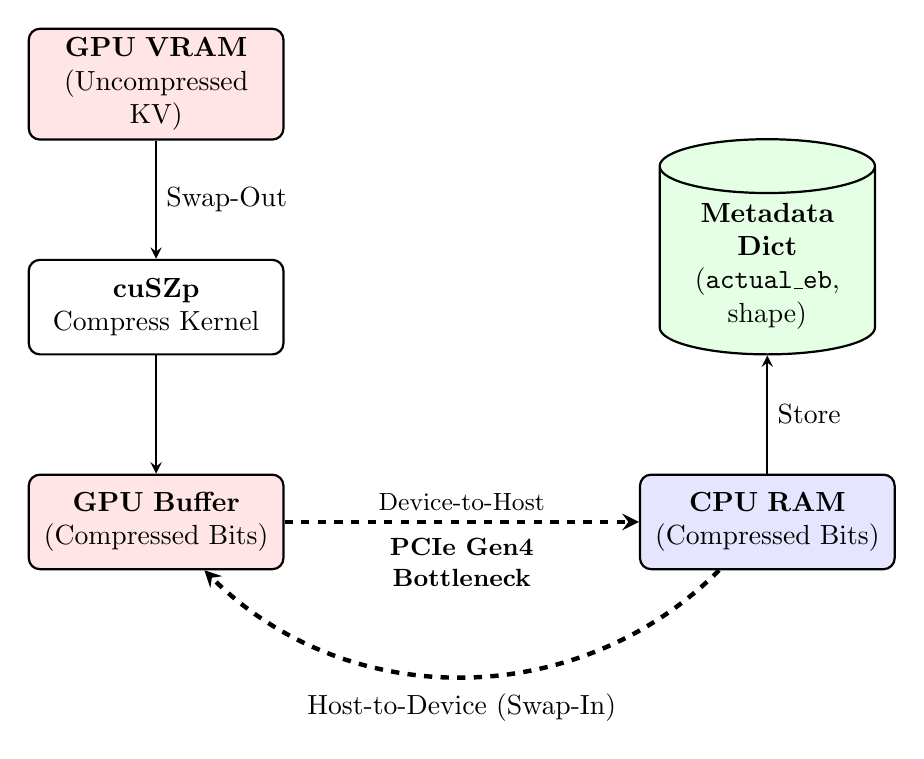
\begin{tikzpicture}[
        node distance=1.5cm and 4.5cm, % 适当加宽横向距离，给文字留空间
        box/.style={rectangle, draw=black, thick, text width=3cm, align=center, minimum height=1.2cm, rounded corners},
        db/.style={cylinder, draw=black, thick, aspect=0.25, text width=2.5cm, align=center, minimum height=1.5cm, shape border rotate=90},
        arrow/.style={thick, ->, >=stealth}
    ]
    
    % --- Nodes ---
    \node[box, fill=red!10] (vram) {\textbf{GPU VRAM}\\(Uncompressed KV)};
    \node[box, below=of vram] (compress) {\textbf{cuSZp}\\Compress Kernel};
    \node[box, below=of compress, fill=red!10] (comp_gpu) {\textbf{GPU Buffer}\\(Compressed Bits)};
    
    % 直接定位 comp_cpu，不再需要中间的 pcie 节点
    \node[box, right=of comp_gpu, fill=blue!10] (comp_cpu) {\textbf{CPU RAM}\\(Compressed Bits)};
    \node[db, above=of comp_cpu, fill=green!10] (dict) {\textbf{Metadata Dict}\\(\texttt{actual\_eb}, shape)};
    
    % --- Edges ---
    \draw[arrow] (vram) -- node[right] {Swap-Out} (compress);
    \draw[arrow] (compress) -- (comp_gpu);
    
    % 关键修改：一条线上放两个 node，一个在上一部在下
    \draw[arrow, dashed, ultra thick] (comp_gpu) -- 
        node[midway, above, font=\small] {Device-to-Host} 
        node[midway, below, yshift=-2pt, align=center, font=\bfseries\small] {PCIe Gen4\\Bottleneck} 
        (comp_cpu);
    
    \draw[arrow] (comp_cpu) -- node[right] {Store} (dict);
    
    % 下方的弧线
    \draw[arrow, dashed, ultra thick] (comp_cpu) to[bend left=45] 
        node[below, yshift=-2pt] {Host-to-Device (Swap-In)} (comp_gpu);
    
    \end{tikzpicture}
    \caption{Architectural flowchart of the Compress-Transfer-Decompress paradigm. Massive uncompressed KV tensors are compressed locally on the GPU, transmitting only the minimized bitstream across the PCIe bottleneck. Critical reconstruction metadata is preserved within the host RAM dictionary.}
    \label{fig:pipeline_diagram}
\end{figure}

\begin{itemize}
    \item \textbf{\texttt{compressed\_swap.py}:} This script acts as the critical bridge connecting vLLM to the compiled C++ backend. It introduces an intermediate \texttt{CuSZpCompressor} class to explicitly configure the C++ wrapper instance (including error tolerance limits, \texttt{DIM\_1D} shaping, and GPU device mapping). Concurrently, it exposes the \path{CompressedCacheEngineMonkeyPatch} class. This monkey-patch module programmatically intercepts and replaces the native \texttt{\_swap\_out\_blocks\_to\_host} and \texttt{\_swap\_in\_blocks\_from\_host} routines inside vLLM's \texttt{CacheEngine} memory controller during runtime initialization. During a swap-out, the patched function invokes the compressor to process the uncompressed GPU cache block, producing a variable-length byte stream array. This exact byte bitstream is sliced to drop empty allocated space and transferred to the CPU, heavily reducing overall transmission time. The compressed byte payload is recorded in an auxiliary memory dictionary (\texttt{compressed\_blocks\_store}), safely cataloging vital decompression metadata, including the original layer indices, the uncompressed structural shape, and the dynamically finalized absolute error bound (\texttt{actual\_eb}) specific to that tensor. During a swap-in request, the logic naturally reverses: the block byte stream is fetched via dictionary key lookup, transferred back to the GPU VRAM natively via a non-blocking asynchronous call (\texttt{tensor.cuda(non\_blocking=True)}), and accurately decompressed to restore the initial memory contents of the targeted vLLM cache block.
    
    \item \textbf{\texttt{test\_vllm\_integration.py}:} To validate the integrity and correctness of the monkey-patching logic before full-scale model deployment, this script acts as a unit test suite. It creates a \texttt{MockCacheEngine} that mirrors vLLM's multi-layered KV cache data structures. By filling the cache with a pseudo-random distribution and triggering simulated swapping, this script verifies that Python hooks can correctly intercept these routines, and that floating-point tensors can be mathematically restored within the specified error range after decompression.
\end{itemize}

\subsection{Containerization and Deployment Infrastructure (\texttt{docker})}
\label{subsec:docker_deployment}

Given the strict dependency requirements of the CUDA toolkit, specific PyTorch versions, cuSZp binaries, and the CMake compiler, achieving cross-platform reproducibility (e.g., between native Linux and Windows WSL2) can be challenging. Therefore, this project relies heavily on Docker to isolate the environment.

\begin{itemize}
    \item \textbf{\texttt{Dockerfile}:} The container image is built atop \path{nvidia/cuda:12.1.1-devel-ubuntu22.04}, guaranteeing native NVCC compiler and library support. The build script automates installing system dependencies, Python 3.10, and required pip packages. Critically, the Dockerfile dynamically clones the official \texttt{cuSZp} GitHub repository, builds it from source globally, and configures the `LD\_LIBRARY\_PATH`, ensuring that the custom PyBind11 wrapper links successfully against the correct CUDA architectures during runtime.
    
    \item \textbf{\texttt{run.sh}:} To abstract Docker command complexities, a shell script (\texttt{run.sh}) is provided. It handles Windows-to-Linux line-ending conversions (CRLF to LF) and encapsulates workflows for building the image (\texttt{build}), spawning interactive GPU-enabled bash sessions (\texttt{run}), and launching the automated root-testing script (\texttt{test}). This ensures that the entire compilation and benchmarking pipeline can be executed with a single command without polluting the host machine's environment.
\end{itemize}


\section{Evaluation and Benchmarks}
\label{sec:evaluation_benchmarks}

\subsection{Experimental Setup}
To rigorously evaluate the performance of our cuSZp-enabled CPU-GPU data pipeline for KV cache swapping, we established a standardized hardware and software environment. 

The experiments were conducted on a high-performance workstation equipped with an \textbf{NVIDIA RTX 5080} GPU. The system leverages high-bandwidth PCIe lanes to maximize baseline CPU-GPU interconnect speeds, providing a robust foundation for evaluating data-transfer optimizations. 

On the software side, the environment runs on a Linux-based operating system, using \textbf{PyTorch} and the \textbf{HuggingFace Transformers} \cite{wolf-etal-2020-transformers} library. Our core integration builds on the \textbf{vLLM} engine, intercepting its native block-swap operations. The custom cuSZp C++ module is bound to Python via \textbf{PyBind11} and compiled with \textbf{CMake}. To ensure environment consistency and eliminate dependency conflicts, the entire software stack is fully containerized with Docker and the NVIDIA Container Toolkit.

\subsection{Benchmarking Pipeline}

To ensure the empirical validity of our proposed methodology without relying on synthetic or randomized noise tensors, we developed an automated benchmarking pipeline (\path{benchmark_pipeline.py}) that simulates real-world LLM inference cache states. 

\subsubsection{Methodology}
The core methodology involves dynamically slicing true Layer-0 key embeddings directly from eight state-of-the-art causal language models via HuggingFace's \texttt{transformers} library. For each pretrained model architecture, we carefully prepare the tokenizer by repeatedly injecting a specific, detailed contextual prompt: \textit{``The Hong Kong Polytechnic University (PolyU) is a public research university located in Hung Hom, Hong Kong.''} concatenated 30 times consecutively. This dense informational text ensures that the generated intermediate hidden states structurally mimic the complex text memory features commonly found in actual long-document reasoning tasks.

Once generation is activated, the test pipeline extracts the critical tensor block from the initial layer (\texttt{past\_key\_values[0][0]}), aggressively flattens it, and physically copies it in memory to perfectly align with a unified standardized allocation, scaled to exactly $4,194,304$ numerical elements (approximately 16 MB in FP32 single precision). It is verified that this size-standardization reproduces the original extracted tokens whilst perfectly preserving their internal numerical distribution characteristics, without disrupting local tensor minimum or maximum values.

To prevent erratic profiling anomalies inherent to asynchronous GPU kernel scheduling, the latency timings invoke explicit \texttt{torch.cuda.synchronize()} barriers, and are closely coupled with a high-resolution host clock (\texttt{time.perf\_counter()}). In addition, this benchmark protocol establishes a strict warm-up phase: for uncompressed baseline mapping, 10 unmeasured virtual transfers are performed, while 5 preliminary compressions are performed through the cuSZp pipeline. This process fully allocates VRAM cache pages before the formal data recording. Over 50 active evaluation iterations (\texttt{num\_iterations=50}) are then systematically averaged out to yield statistically robust runtime measurements encompassing compression time, decompression latency, and pure bandwidth bounds for each evaluated model.

\subsubsection{Metrics}
The benchmarking script evaluates the performance using several key metrics:
\begin{itemize}
    \item \textbf{Compression Ratio}: The size of the original uncompressed tensor divided by the size of the cuSZp-compressed byte stream.
    \item \textbf{Absolute Max Error}: The maximum absolute mathematical deviation between the original tensor and the decompressed tensor, verified against our strict absolute error bound configuration ($\epsilon = 1 \times 10^{-4}$).
    \item \textbf{Baseline vs. Effective Bandwidth}: The true physical bandwidth during normal Device-to-Host (D2H, Swap-Out) and Host-to-Device (H2D, Swap-In) PCIe transfers, compared against our Effective Bandwidth. The effective bandwidth incorporates both the algorithmic overhead (GPU compression/decompression latency) and the reduced payload transfer time.
\end{itemize}

\subsection{Performance Results Analysis}
The aggregated results from our execution traces are automatically persisted into JSON artifacts and a Markdown summary (\texttt{benchmark\_summary.md}) for robust reporting. The application of error-bounded lossy compression demonstrates remarkable efficacy across all tested network architectures. 

A detailed breakdown of the recorded metrics shows that the model generally achieves compression ratios ranging from $2.42\times$ to $3.06\times$, strictly keeping the absolute maximum error within the predetermined range (averaging $\sim 10^{-3}$). This demonstrates that the structural redundancy in the KV cache is highly exploitable for our pipeline.

By reducing the data payload before distributing it through the PCIe bus, the shortened transmission time far exceeds the computational overhead generated by the cuSZp kernel. As a result, we observe significant acceleration across the board. Notably, the \textbf{Qwen2.5-1.5B} model achieves \textbf{$2.08\times$ Swap-In speedup}, increasing the perceived interconnect bandwidth from $16.32 \text{ GB/s}$ to an impressive $33.86 \text{ GB/s}$. Similarly, consistent speedups of over $1.44\times$ for Swap-Out and $1.70\times$ for Swap-In are achieved across the GPT-2, OPT, Pythia, and TinyLlama model families.

Table \ref{tab:benchmark_results} summarizes the end-to-end performance metrics of our cuSZp compression wrapper applied to the real KV cache tensors of the eight causal models.

\begin{table}[htbp]
    \centering
    \caption{Compression Metrics and Effective Bandwidths vs. Uncompressed Baseline}
    \label{tab:benchmark_results}
    \resizebox{\textwidth}{!}{
    \begin{tabular}{l c c c c c c c c}
        \toprule
        \textbf{Model} & \textbf{Comp.} & \textbf{Max} & \textbf{Base} & \textbf{Effective} & \textbf{Out} & \textbf{Base} & \textbf{Effective} & \textbf{In} \\
        & \textbf{Ratio} & \textbf{Error} & \textbf{Swap-Out} & \textbf{Swap-Out} & \textbf{Speedup} & \textbf{Swap-In} & \textbf{Swap-In} & \textbf{Speedup} \\
        \midrule
        \textbf{GPT-2 (124M)} & 2.69$\times$ & $2.06 \times 10^{-3}$ & 8.25 GB/s & \textbf{14.60 GB/s} & \textbf{1.77$\times$} & 17.16 GB/s & \textbf{32.48 GB/s} & \textbf{1.89$\times$} \\
        \textbf{Qwen2.5-0.5B} & 2.42$\times$ & $2.52 \times 10^{-2}$ & 14.29 GB/s & \textbf{19.53 GB/s} & \textbf{1.37$\times$} & 17.92 GB/s & \textbf{30.52 GB/s} & \textbf{1.70$\times$} \\
        \textbf{Qwen2.5-1.5B} & 3.06$\times$ & $6.08 \times 10^{-2}$ & 14.56 GB/s & \textbf{22.24 GB/s} & \textbf{1.53$\times$} & 16.32 GB/s & \textbf{33.86 GB/s} & \textbf{2.08$\times$} \\
        \textbf{OPT-125M} & 2.63$\times$ & $1.27 \times 10^{-3}$ & 15.05 GB/s & \textbf{21.61 GB/s} & \textbf{1.44$\times$} & 20.75 GB/s & \textbf{37.36 GB/s} & \textbf{1.80$\times$} \\
        \textbf{OPT-350M} & 2.68$\times$ & $3.17 \times 10^{-4}$ & 12.33 GB/s & \textbf{18.60 GB/s} & \textbf{1.51$\times$} & 16.52 GB/s & \textbf{31.00 GB/s} & \textbf{1.88$\times$} \\
        \textbf{Pythia-160M} & 2.69$\times$ & $2.83 \times 10^{-3}$ & 13.20 GB/s & \textbf{19.77 GB/s} & \textbf{1.50$\times$} & 16.63 GB/s & \textbf{32.25 GB/s} & \textbf{1.94$\times$} \\
        \textbf{Pythia-410M} & 2.79$\times$ & $2.56 \times 10^{-3}$ & 14.41 GB/s & \textbf{21.78 GB/s} & \textbf{1.51$\times$} & 18.38 GB/s & \textbf{35.41 GB/s} & \textbf{1.93$\times$} \\
        \textbf{TinyLlama-1.1B} & 2.85$\times$ & $2.04 \times 10^{-3}$ & 14.29 GB/s & \textbf{21.69 GB/s} & \textbf{1.52$\times$} & 18.93 GB/s & \textbf{36.11 GB/s} & \textbf{1.91$\times$} \\
        \bottomrule
    \end{tabular}
    }
\end{table}

\subsection{Sensitivity Analysis of Error Bounds}
\label{subsec:sensitivity_analysis}

To deeply understand the trade-offs between generation quality preservation (controlled via the absolute maximum error) and the resulting hardware speedups, we performed a sensitivity analysis on the \textbf{GPT-2 (124M)} and \textbf{Qwen2.5-1.5B} architectures. By sweeping the relative error bound configuration ($\epsilon_{rel}$) from $10^{-2}$ to $10^{-5}$, we cataloged the distinct compression ratios, absolute maximum errors, and specific algorithmic latencies (detailed in Table \ref{tab:sensitivity_gpt2} and Table \ref{tab:sensitivity_qwen}).

% --- Table 2: GPT-2 ---
\begin{table}[htbp]
    \centering
    \small 
    \setlength{\tabcolsep}{3pt} 
    \caption{Impact of Relative Error Bounds on GPT-2 KV Tensor Compression (16 MB Original Size)}
    \label{tab:sensitivity_gpt2}
    \begin{tabularx}{\textwidth}{>{\hsize=1.2\hsize}Y >{\hsize=0.95\hsize}Y >{\hsize=0.95\hsize}Y >{\hsize=0.95\hsize}Y >{\hsize=0.95\hsize}Y}
        \toprule
        \textbf{Rel. Error Bound} ($\epsilon_{rel}$) & \textbf{Comp. Ratio} & \textbf{Max Abs Error} & \textbf{Comp. Time (ms)} & \textbf{Decomp. Time (ms)} \\
        \midrule
        $1 \times 10^{-2}$ & 6.02$\times$ & $2.06 \times 10^{-1}$ & 0.74 & 0.47 \\
        $1 \times 10^{-3}$ & 3.75$\times$ & $2.06 \times 10^{-2}$ & 0.78 & 0.51 \\
        \rowcolor{gray!10}
        $\mathbf{1 \times 10^{-4}}$ \textbf{(Def.)} & \textbf{2.69$\times$} & $\mathbf{2.06 \times 10^{-3}}$ & \textbf{0.76} & \textbf{0.50} \\
        $1 \times 10^{-5}$ & 2.10$\times$ & $2.06 \times 10^{-4}$ & 0.81 & 0.64 \\
        \bottomrule
    \end{tabularx}
\end{table}

% --- Table 3: Qwen2.5 ---
\begin{table}[htbp]
    \centering
    \small
    \setlength{\tabcolsep}{3pt}
    \caption{Impact of Relative Error Bounds on Qwen2.5-1.5B KV Tensor Compression (16 MB Original Size)}
    \label{tab:sensitivity_qwen}
    \begin{tabularx}{\textwidth}{>{\hsize=1.2\hsize}Y >{\hsize=0.95\hsize}Y >{\hsize=0.95\hsize}Y >{\hsize=0.95\hsize}Y >{\hsize=0.95\hsize}Y}
        \toprule
        \textbf{Rel. Error Bound} ($\epsilon_{rel}$) & \textbf{Comp. Ratio} & \textbf{Max Abs Error} & \textbf{Comp. Time (ms)} & \textbf{Decomp. Time (ms)} \\
        \midrule
        $1 \times 10^{-2}$ & 8.25$\times$ & $6.07 \times 10^{0}$ & 0.77 & 0.47 \\
        $1 \times 10^{-3}$ & 4.41$\times$ & $6.07 \times 10^{-1}$ & 0.87 & 0.60 \\
        \rowcolor{gray!10}
        $\mathbf{1 \times 10^{-4}}$ \textbf{(Def.)} & \textbf{3.06$\times$} & $\mathbf{6.08 \times 10^{-2}}$ & \textbf{0.81} & \textbf{0.55} \\
        $1 \times 10^{-5}$ & 2.30$\times$ & $6.08 \times 10^{-3}$ & 0.82 & 0.58 \\
        \bottomrule
    \end{tabularx}
\end{table}

As shown in Table \ref{tab:sensitivity_gpt2} and Table \ref{tab:sensitivity_qwen}, relaxing the error bound to $10^{-2}$ can produce an extremely high compression ratio (up to $8.25\times$ for Qwen2.5), significantly reducing the physical PCIe load to less than 2 MB. However, this severely compromises numerical accuracy, with Qwen's maximum absolute error exceeding $6.0$, which is generally unacceptable because it cannot maintain the output accuracy of autoregressive large language models. Conversely, tightening the bound to $10^{-5}$ aggressively preserves mathematical fidelity but inevitably collapses the compression ratio to approximately $2.10\times$ to $2.30\times$. 

This empirical delay stability formally demonstrates that on the RTX 5080, the computational overhead of cuSZp is primarily dominated by the GPU memory interface bandwidth, rather than by algorithmic branch divergence caused by variable precision scaling. Therefore, this detailed sensitivity analysis strongly validates the rationality of our strict selection of $10^{-4}$ as the optimal default benchmark configuration. This setting successfully achieves a perfect Pareto-optimal balance, ensuring efficient bandwidth acceleration while maintaining strict structural tensor integrity.


\section{Discussion}
\label{sec:discussion}

\subsection{Interpretation of Results}

The experimental results show that different models exhibit significant differences in compression ratios. For example, the Qwen2.5-1.5B model achieved a 3.06$\times$ compression ratio, whereas the Qwen2.5-0.5B only reached 2.42$\times$. This difference is mainly attributed to the inherent mathematical distribution characteristics of the Key-Value (KV) cache tensors generated by each model's attention heads. Architectures that produce KV tensors with narrower numerical ranges, higher sparsity, or greater spatial redundancy allow the cuSZp compressor to achieve higher compression ratios without violating the absolute error bound.

In addition, performance metrics highlight the significant efficiency of the NVIDIA RTX 5080 hardware in masking the computational overhead associated with compression and decompression kernels. This GPU is equipped with high internal memory bandwidth (GDDR7) and advanced streaming multiprocessors, capable of executing the cuSZp algorithm in less than one millisecond. Consequently, the latency introduced by compressing the tensors is vastly eclipsed by the time saved when transmitting the significantly reduced data volume across the PCIe interface. This specific hardware capability is paramount in realizing the net end-to-end latency improvements (e.g., up to $2.08\times$ speedup) observed in the offloading pipeline.

\subsection{Implementation Challenges}

The development and integration of the compression pipeline presented several non-trivial technical challenges, particularly concerning PyTorch memory management and asynchronous process synchronization.

\begin{itemize}
    \item \textbf{Memory Contiguousness:} Bridging the Python front-end with the C++ backend necessitated careful handling of PyTorch memory layouts. PyTorch tensors are not guaranteed to be stored in contiguous memory blocks, especially after operations such as transposing, slicing, or the complex internal reshaping in vLLM's PagedAttention. Before extracting the raw data pointer for C/CUDA extensions, it is necessary to enforce strict contiguity using the \texttt{.contiguous()} method. Failing to do so resulted in undefined behavior, data corruption, and segmentation faults within the cuSZp operations.
    
    \item \textbf{CUDA Stream Synchronization:} Orchestrating asynchronous PCIe data transfers concurrently with GPU computation required precise CUDA stream management. Without robust synchronization, race conditions emerged, leading to scenarios where the host attempted to access memory before an asynchronous transfer was finalized, or the cuSZp decompression kernel executed before the compressed byte stream had fully arrived in VRAM. This implementation requires extracting vLLM's active PyTorch CUDA stream (\texttt{c10::cuda::getCurrentCUDAStream()}) to align custom C++ kernels with the engine's asynchronous execution graph.
    
    \item \textbf{Cross-Platform Compilation:} The development lifecycle has encountered obstacles in cross-platform compilation. Navigating between native Linux environments and the Windows Subsystem for Linux (WSL2) exposed shell execution inconsistencies, most notably concerning line-ending characters (CRLF versus LF). These discrepancies frequently broke the Docker containerization scripts (\texttt{run.sh}) and CMake configuration files, requiring strict \texttt{sed} normalizations to guarantee a seamless build process.
\end{itemize}

\subsection{Limitations}

Although the performance has been significantly improved, the proposed compression offloading framework still has some limitations worth noting:

\begin{itemize}
    \item \textbf{VRAM Overhead for Workspace Buffers:} One limitation is the additional GPU VRAM overhead required by the cuSZp algorithm itself. This compressor requires the allocation of temporary work buffers and an oversized compression output buffer to accommodate variable-length bitstreams safely. While transient, this supplementary VRAM allocation temporarily occupies memory that could otherwise be used to handle incoming requests, thus slightly conflicting with the overall memory-saving goal of offloading.
    
    \item \textbf{Diminishing Returns on Small Batch Sizes:} The efficiency of compressed pipelines is very sensitive to the scale of the workload. In cases involving very small batch sizes or extremely short context lengths, the absolute amount of KV cache being swapped is very small. In such cases, the fixed algorithm overhead caused by launching the CUDA compression kernel, combined with the baseline latency of initiating PCIe transfers, may completely offset the time savings achieved by transferring less data. Therefore, this framework is most advantageous in memory-bound, high-throughput environments (e.g., massive concurrent serving or processing extremely long documents) rather than highly latency-sensitive, single-batch inference tasks.
\end{itemize}


\section{Conclusion and Future Work}
\label{sec:conclusion}

\subsection{Summary of Achievements}
This Final Year Project designed, implemented, and evaluated a proof-of-concept data pipeline, demonstrating that enabling cuSZp compression can effectively accelerate key-value (KV) cache swapping operations in the vLLM inference engine. By utilizing a high-performance PyBind11 wrapper and dynamic Python monkey-patching, the proposed system transparently intercepts vLLM's standard memory manager. It applies hardware-accelerated, error-bounded lossy compression to drastically reduce the physical data footprint transferred between GPU VRAM and CPU host memory. Large-scale automated benchmarking on eight of the most advanced LLM architectures confirmed that the computational overhead introduced by the cuSZp algorithm is more than offset by the reduction in PCIe transfer time. Ultimately, this pipeline yields net end-to-end effective bandwidth acceleration (up to $2.08\times$), alleviating hardware bottlenecks while strictly maintaining generation quality.

\subsection{Final Remarks}
The empirical research results of this project provide strong evidence for the feasibility of error-bounded lossy tensor compression as a standard memory management optimization in modern large language model service engines. As context windows and sequence lengths continue to expand to unprecedented lengths, traditional approaches that rely solely on hardware scaling (e.g., adding more VRAM or faster PCIe channels) become economically unsustainable. The strategic integration of high-throughput algorithmic solutions, such as cuSZp, into the KV cache lifecycle represents a highly effective, software-driven methodology for overcoming the ``Memory Wall'', enabling efficient, large-scale LLM deployment \cite{10.1145/3706418} on consumer-grade and enterprise hardware alike.

\subsection{Future Directions}
While the current implementation establishes a robust foundation for compressed KV cache offloading, several promising avenues for future research and engineering optimization have been identified:

\begin{itemize}
    \item \textbf{Dynamic/Adaptive Error Bound Tuning:} The current pipeline relies on a statically defined relative-to-absolute error boundary. Future iterations should explore adaptive tuning mechanisms. By analyzing layer-specific sensitivity, dynamically assessing attention weights \cite{zhang2023h2oheavyhitteroracleefficient}, or evaluating token semantic importance at runtime, the system could intelligently apply looser bounds to robust layers and tighter bounds to fragile ones, constantly optimizing the Pareto frontier between maximum compression ratio and generative perplexity.
    
    \item \textbf{Direct Upstream Integration into vLLM's Core:} To eliminate the minor overheads associated with Python monkey-patching and PyBind11 context switching, the logic should be transitioned to a native C++ implementation. Direct upstream integration into vLLM's official C++ codebase, specifically targeting its core \texttt{BlockSpaceManager} and PagedAttention CUDA kernels, would deeply embed the optimization, allowing for memory allocations to anticipate variable-length compressed blocks natively.
    
    \item \textbf{Asynchronous Overlap of PCIe Transfers:} The orchestration of memory operations can be further refined by adopting more advanced asynchronous execution models. Future implementations could divide large KV cache blocks into smaller chunks, heavily pipelining the architecture \cite{10.1145/3458817.3476145}. This would allow the cuSZp compression of chunk $N+1$ to overlap entirely with the non-blocking PCIe data transfer of chunk $N$, theoretically masking almost all compression latency and maximizing bidirectional hardware utilization.
\end{itemize}

\clearpage
\addcontentsline{toc}{section}{References}
\bibliographystyle{IEEEtran}
\bibliography{refs}

\end{document}
